\section{Experimental Setup}

We have described details of the experimental setup in ref.\cite{Araoka:2011pw},
and in this paper we only discuss the issues which are relevant.

\subsection{K1.1Br Beamline}
K1.1Br beamline is located at J-PARC slow extraction facility.
It is designed and constructed for TREK experiment~\cite{ref:TREK}. 
to obtain high intensity and high purity $K^+$ beam with momentum around 800 MeV/$c$.
30 GeV/$c$ protons are irradiated to production target, and bending magnets
and an electo-static separator (ESS) provide excelent momentum separation and mass separation, respectively.
Other than $K^+$, Protons and $\pi^+$ and $e^+$ are also available in this beamline. 
While October 2010 run period, using 3.6 kW of 30 GeV/$c$ proton on target, 
TREK collaboration have achieved $K/\pi$ ratio of $\sim$1 with Kaon rate of $\sim$1 kHz.
For LArTPC test, we have intentionally reduced the beam intensity to $\sim$ 10 Hz 
to avoid particle overwrap, and maximum achived  $K/\pi$ with this condition was $\sim$1/4.

800 Mev/$c$ $\pi^+$ and $K^+$ are passing-through the 250L TPC detector.
We reduce their momentum to $\sim$600 MeV/$c$ and $\sim$200 MeV/$c$, respetcively,
so that they stop inside the TPC fiducial volume.
200 MeV/$c$ $\pi^+$ is obtained by changing the beamline optics and turning off ESS,
because $\pi^+$(and $e^+$) is dominant component without ESS.
To obeain 600 MeV/$c$ $K^+$, a beam degrader is located at downstream of the beamline
and $K^+$ lose its enery by ionization.We use a combination of lead glass blocks (LG) 
and lead brick (LB) as beam degrader with thckness of 12.5 cm and 2.5 cm, respectively.

\subsection{250L Detector}

The cryostat..

The TPC we have build for this test is a simple grid chamber
with active volume of 40 cm$\times$ 40 cm$\times$ 76 cm$\times$.

Cathode plane and anode plane is located at 
at the bottom and top of the field cage, respectively,
and grid plane is inserted 1 cm from the anode plane.
Side of the TPC us surrounded by field shapers.

The cathode and grid planes are 100 $\mu$m stainless steel wire
spaced by 5 mm.

The Anode is made with PCB (printed circuit board) with readout pitch of 1 cm.
Substrate of PCB is 1.6 mm FR-4 glass-rainforced epoxy
and electrode is 100 $\mu$m of gold-plated copper.

The field shaper is also made with PCB


The charge

12 bit ADC with 2.5 MHz sampling frequency

\subsection{Beamline Equipment}

We have several beam counters to identify beam particles.
% (see Fig\ref{fig:Beamline}).
There are two beam defining counters (BDC and T32 BDC) which determine acceptance of the beam, 
a Fitch-type Cherenkov counter (FC), and a Gas Cherenkov counter (GC), 
and two time of flight counters (TOF1 and TOF2).

%\begin{figure}[htbp]
%  \centering
%  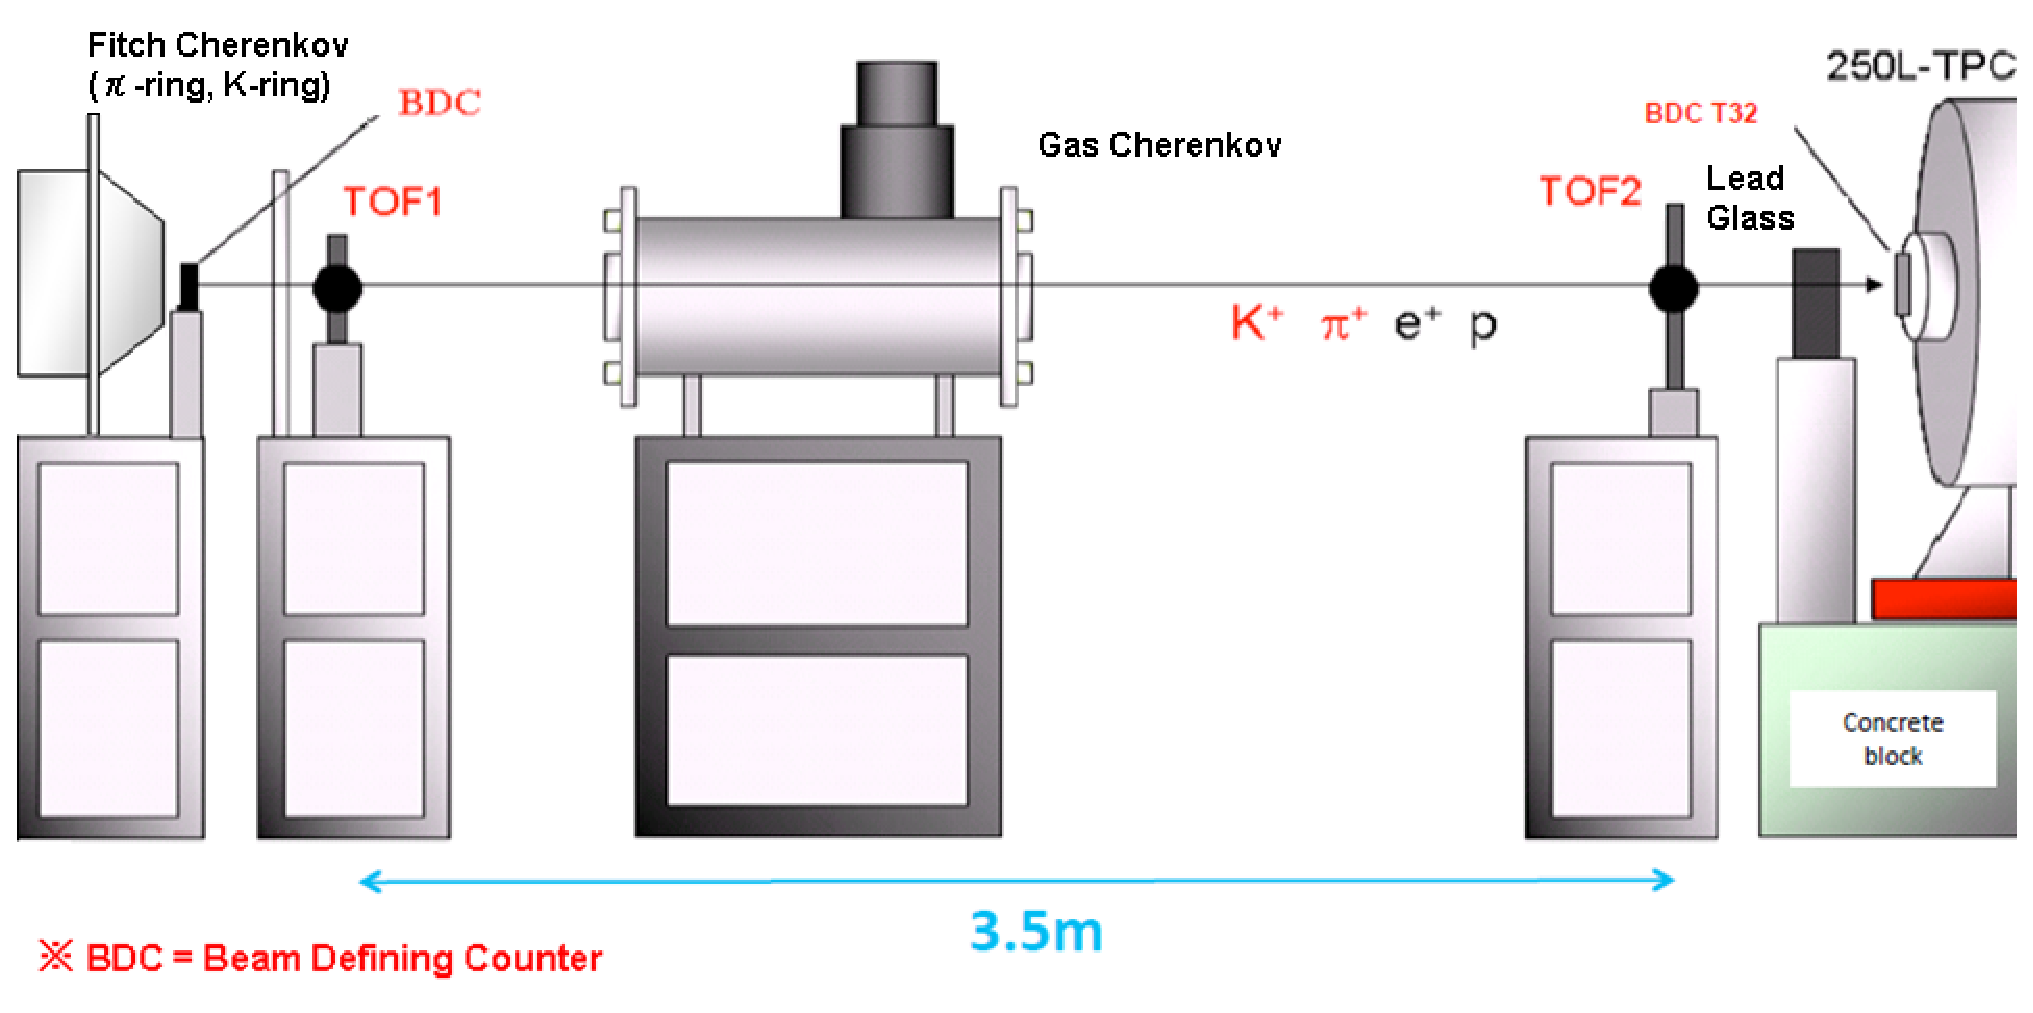
\includegraphics[width=1.0\hsize,clip]{fig/Beamline.eps}
%  \caption{Instruments on K1.1BR Beam Line}
%  \label{fig:Beamline}
%\end{figure}

Two TOF counters are about 3.5m apart, and time resolution is abot $\sim$200 ps.
Figure \ref{fig:BeamCountersTOF} shows the flight time distribution between TOF1 and TOF2
obtained from 800 MeV/$c$ beam particles which contain  $K^{+}$, $\pi{+}$, $e^{+}$, and $p$. 
Three peaks which correspond to $\pi$+$e^+$, $K^+$, and $p$, respectively, are well separated.
FC has 4 cm of acrylic plate as Cherenkov light radiator and 
photo-multipliers which are aligned in circles with two different emission angles
($K$-ring and $\pi$-ring) as photo detector. It is designed to have maximum separation of 
$K^{+}$ and $\pi^{+}$ with momentum of 800 MeV/$c$.
Top plot in Fig.\ref{fig:BeamCountersFC} shows response of FC for the 800 MeV/$c$ beam particles. 
Horizontal axis and vertical axis are hit multiplicity of the $\pi$-ring and $K$-ring, respectively. 
$K^+$($\pi$) is identified as event with signal in $K$-ring ($\pi$-ring) but no signal in $\pi$-ring ($K$-ring).
In case of no signals in both rings, the particle is considered as proton.
Additional separation between $e^{+}$ from $\pi^+$ is provided by GC 
which uses atmospheric air as Cherenkov radiator. 
Filled histograms in bottom plot of Fig.\ref{fig:BeamCounters} shows selected $K^+$ event with FC information.
After removing residual $\pi^+$ using TOF, $K^+$ sample is almost 100\% purity.

\begin{figure}[htbp]
  \begin{center}
    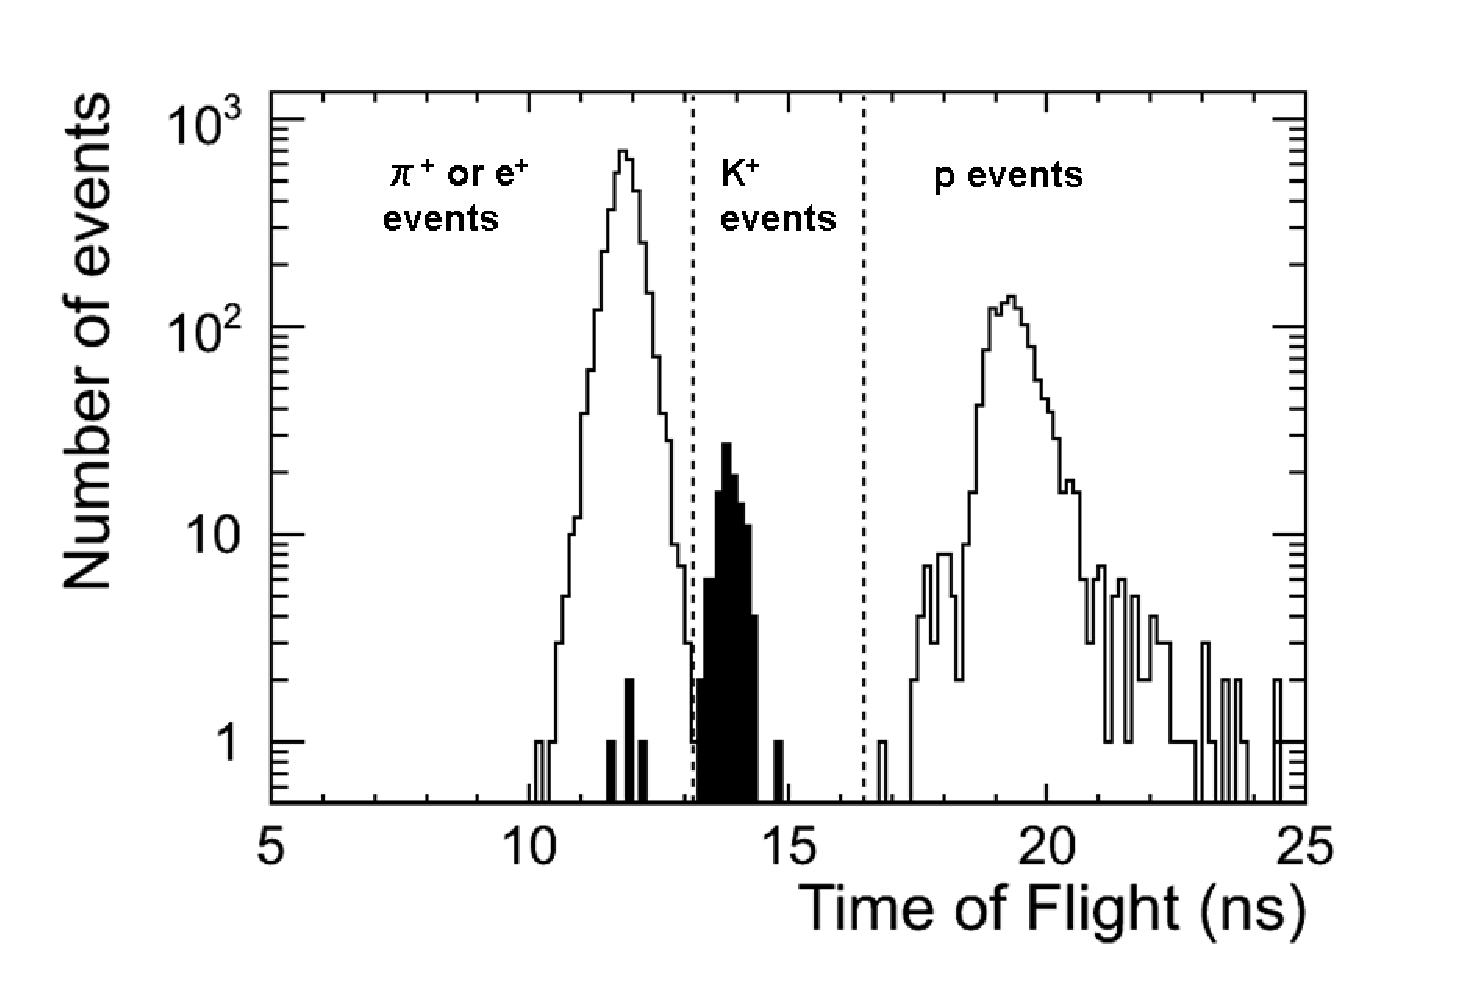
\includegraphics[width=1.0\hsize,clip]{fig/TOF_cut.eps}
  \end{center}
 \caption{TOF distribution.}
 \label{fig:BeamCountersTOF}
\end{figure}

\begin{figure}[htbp]
  \begin{center}
    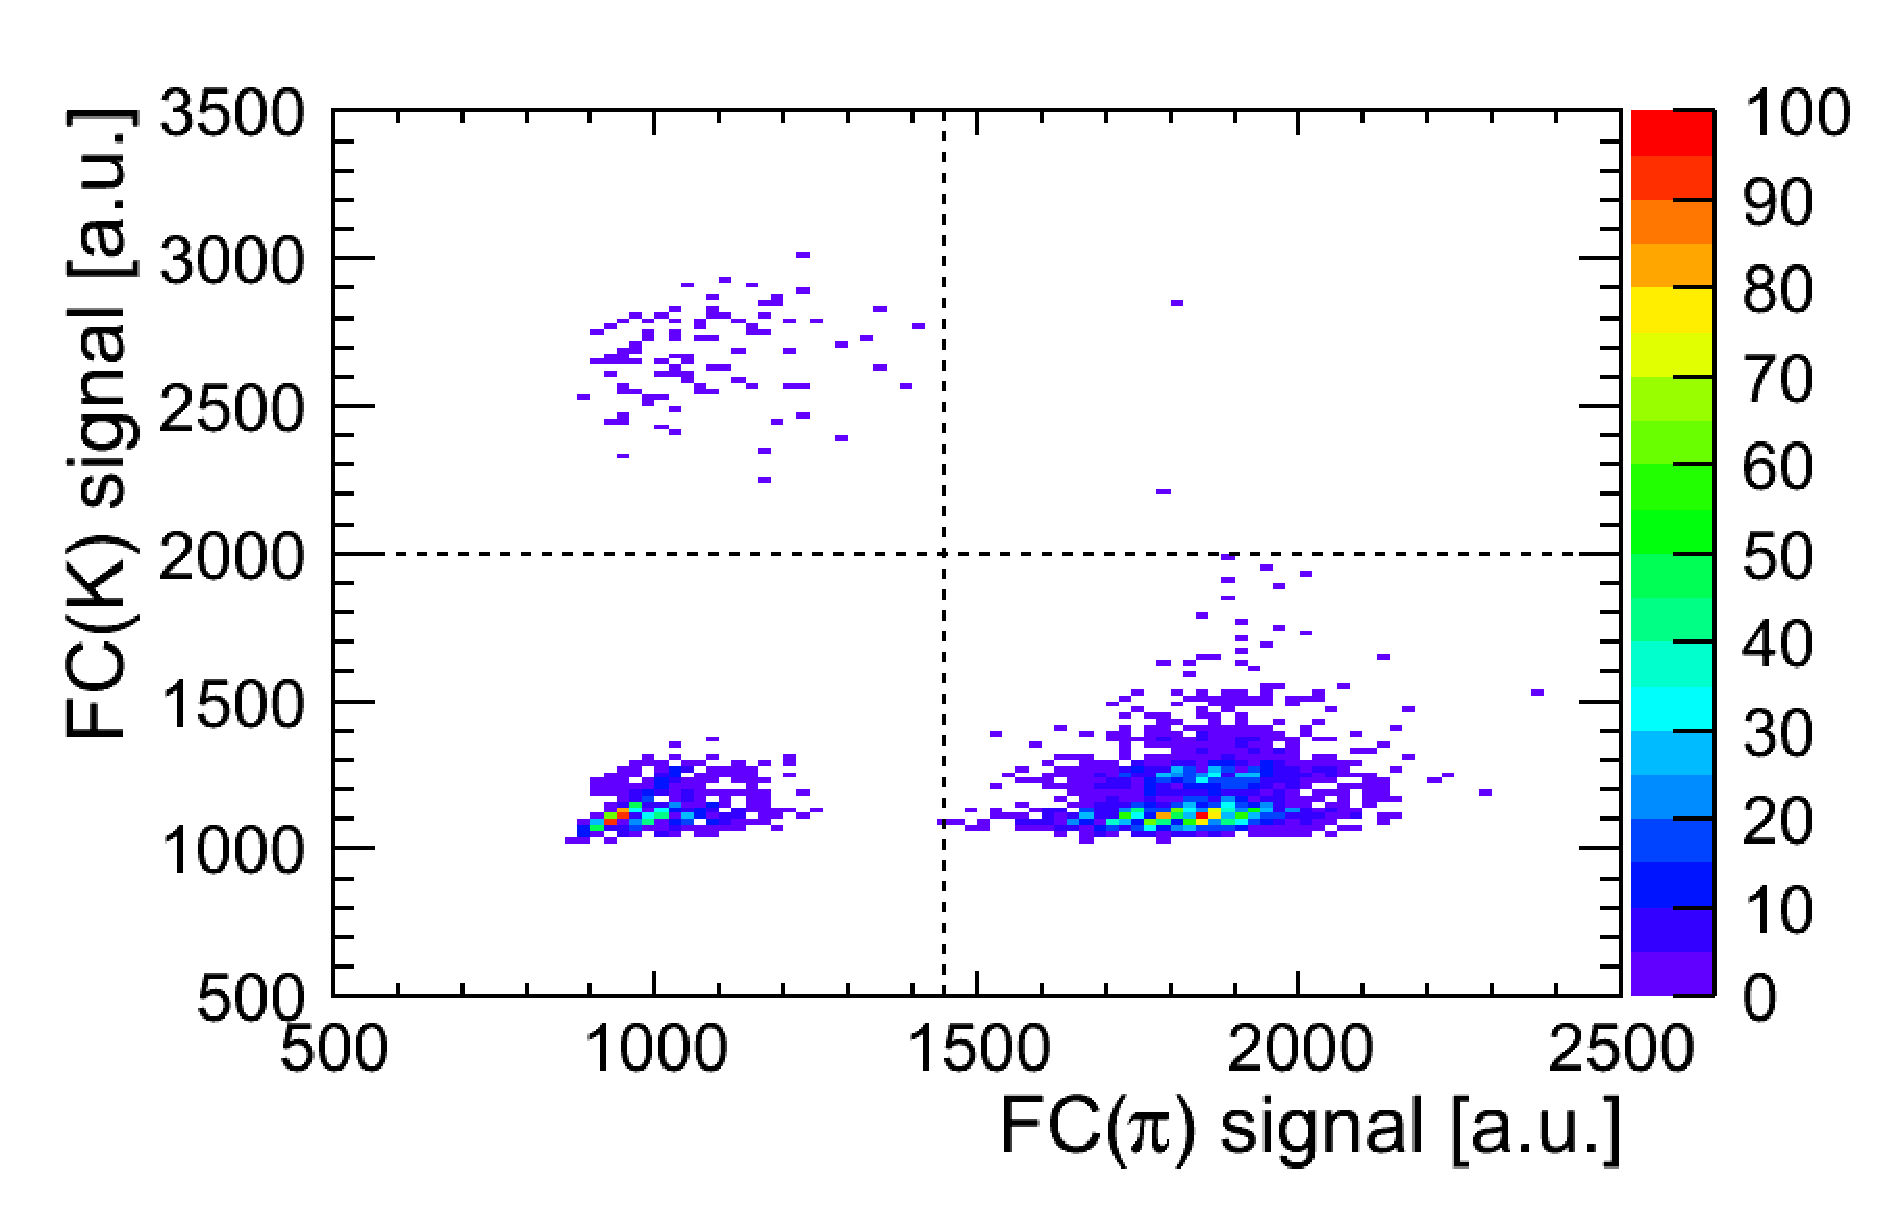
\includegraphics[width=1.0\hsize,clip]{fig/FC_KPI.eps}
  \end{center}
 \caption{FC}
 \label{fig:BeamCountersFC}
\end{figure}


\subsection{Oct/2010 Beam Test Configuration}

by using the beam counters, we define three types of triggers:
(i) non-bias trigger simply requires signal in two BDCs and two TOFs;
(ii) Kaon trigger requires, in addition to non-bias trigger, K identification with FC information;
(iii) electron trigger rquires, in addition to non-bias trigger, electron identification with GC information.

Beam Momentum
\begin{itemize}
\item Materials located from proton target to LArTPC detector (beam counters, beam windows, air, etc) degrade beam particle momentum
\item the effect is estimated by looking at TOF of proton, average prton beam momentum is 730 MeV/$c$
\item For other particles  (K, pi,e e), TOF does not have enough resolution to determin momentum, and the degradation
is directly estimated by counting the energy deposition to the materials using GEANT based simulation.
For example Kaon momentum is xxx MeV/c on average.
\end{itemize}

\begin{figure}[htbp]
  \begin{center}
    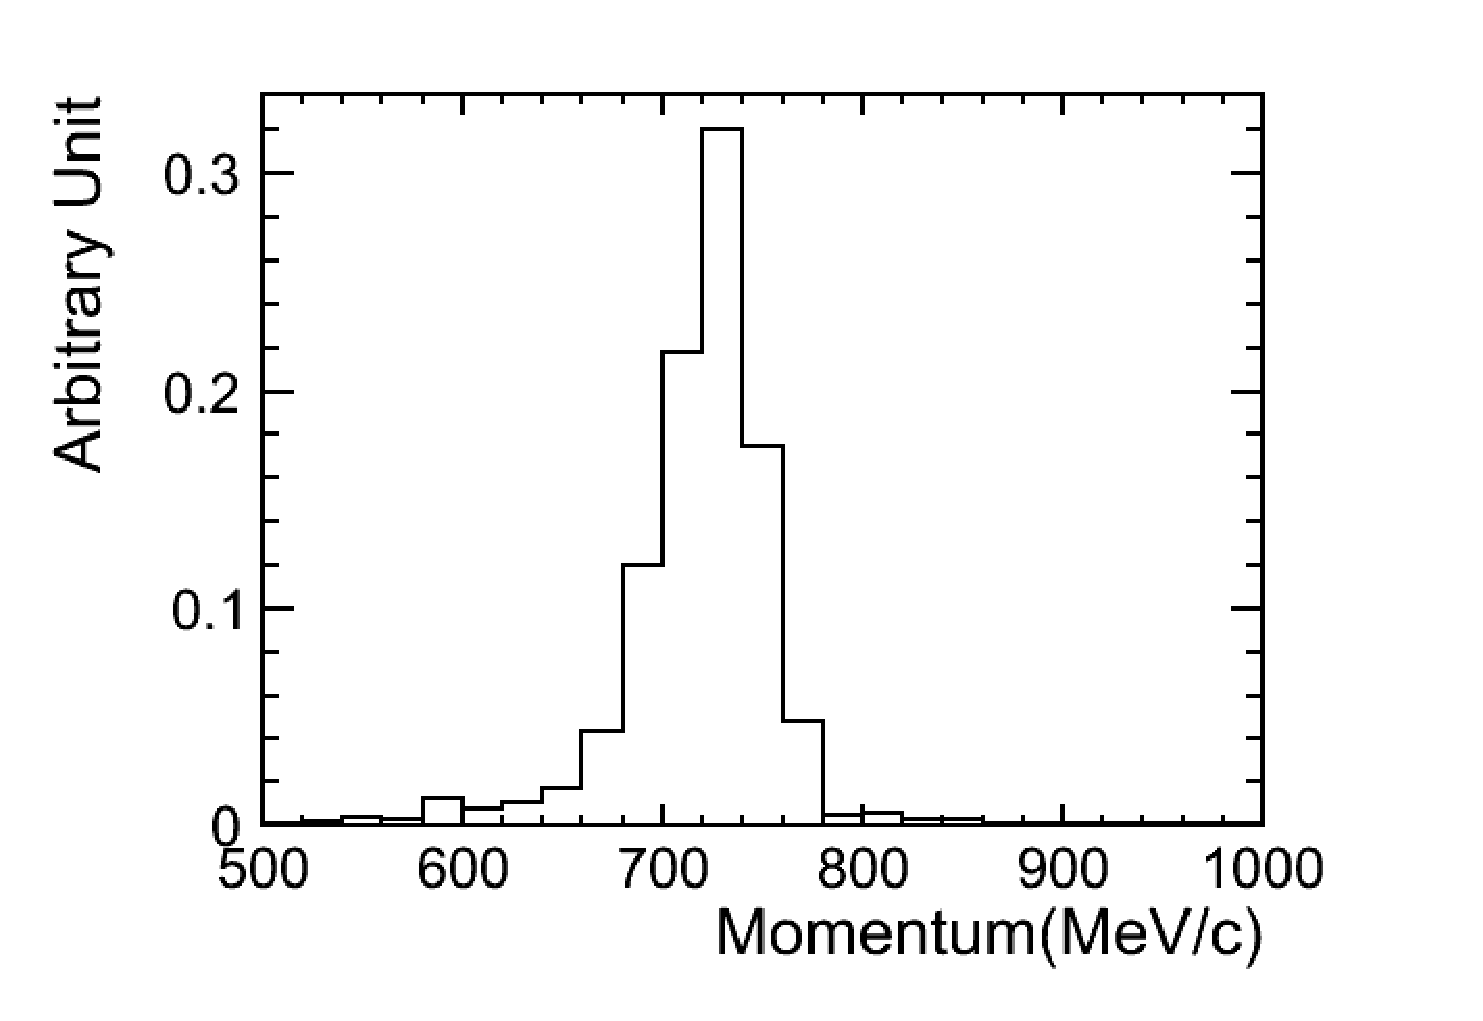
\includegraphics[width=1.0\hsize,clip]{fig/Momentum_proton.eps}
    \caption{Top plot shows $\rm {\Delta TOF}$ distribution of TOF counters with proton data,
      and bottom plot shows proton momentum estimated by $\rm {\Delta TOF}$ of TOF counters information}
    \label{fig:Proton_momentum}
  \end{center}
\end{figure} 

We measured beam profile in front of 250LAr TPC beam window by using plastic scintillation counters.
%Figure \ref{beamprofile_250L} shows the result.
The beam is relatively narrow in vertical direction (within 5 cm),
but spread in horizontal direction ($\sim$ 10 cm).

%\begin{figure}[!htb]
%  \begin{center}
%     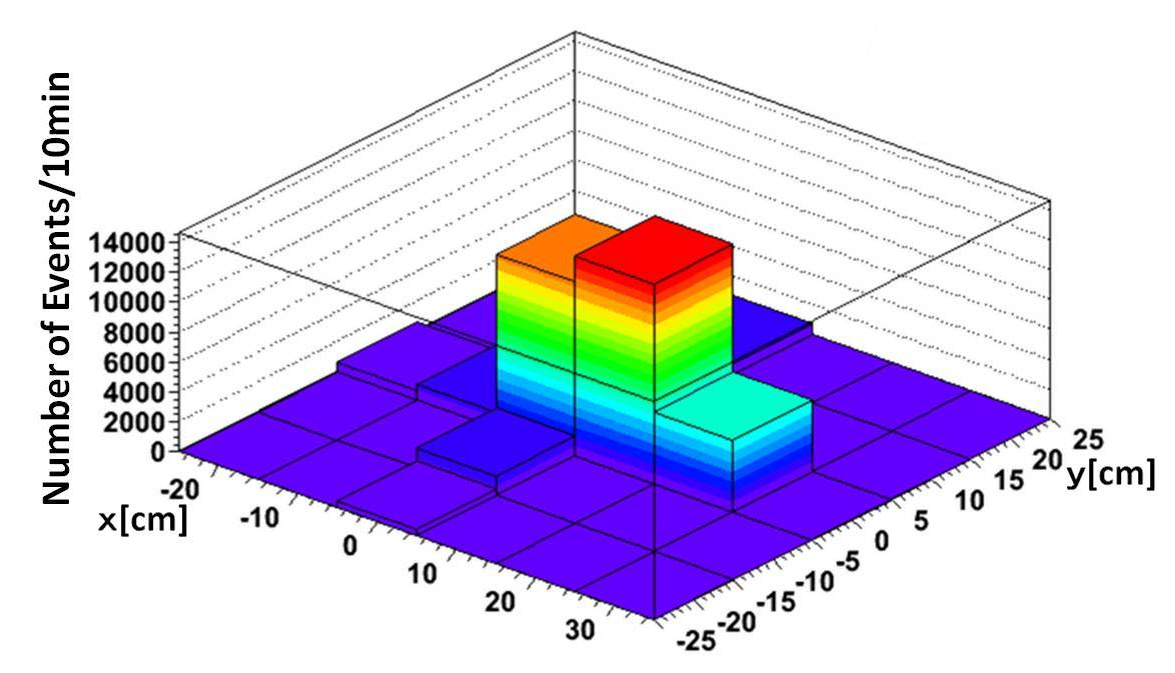
\includegraphics[width=0.8\hsize,clip]{./fig/BeamProfile3.eps}
%  \end{center}
%  \caption{Beam profile on the front of 250LAr TPC}
%  \label{beamprofile_250L}
%\end{figure}


